%%%%%%%%%%%%%%%%%%%%%%%%%%%%%%%%%%%%%%%%%%%%%%%%%%%%%%%%%%%%%%%
%
% Welcome to Overleaf --- just edit your LaTeX on the left,
% and we'll compile it for you on the right. If you open the
% 'Share' menu, you can invite other users to edit at the same
% time. See www.overleaf.com/learn for more info. Enjoy!
%
%%%%%%%%%%%%%%%%%%%%%%%%%%%%%%%%%%%%%%%%%%%%%%%%%%%%%%%%%%%%%%%


% Inbuilt themes in beamer
\documentclass[15pt]{beamer}


% Theme choice:
\usetheme{Warsaw}
\usecolortheme{rose}

% Title page details: 
\title{Assignment-10} 
\author{Shivanshu  Ai21btech11027}
\date{june 10, 2022}
\begin{document}
\begin{frame}
    \titlepage 
\end{frame}

\begin{frame}{Outline}
    \tableofcontents
\end{frame}

    \section{Question}
    \begin{frame}{Question}
        \textbf{Papoulis book exercise 6}\\
        \large \noindent Q-39 The process x(t) is real with autocorrelation R($\tau$).\\
        (a) Show that \\
        \begin{center}
             P\{$|$x(t + $\tau$) - x(t)$| \geq a$ \} $\leq 2[R(0) - R(\tau$)]/$a^2$
        \end{center}
        (B) Express P\{$|$x(t + $\tau$) - x(t)$| \geq a$ \} in terms of the second-order density of x(t).\\
    \end{frame}
    \section{Solution}
    \begin{frame}{Solution}
        (a) As we know for any $\epsilon > 0$,
        \begin{center}
            \begin{align}
                P\{|x - \eta| \geq \epsilon \} \leq \dfrac{\sigma^2}{\epsilon^2}
            \end{align}
        \end{center}
        with $x = x(t + r) - x(t)$ and also from (8 - 101):
        \begin{align}
            P\{|x(t + \tau) - x(t)| \geq a \} &\leq \dfrac{2[R(0) - R(\tau)]}{a^2} \\
            &= 2[R(0) - R(\tau)]/a^2
        \end{align}
    \end{frame}
    \begin{frame}
        (b)
        The above probability equals the mass in the region (shaded) $x_2 - x_1 > a$ and $x_2 - x_1 < -a$.\\
        Hence,
    \end{frame}
    \begin{frame}
        \begin{figure}[h]
            \centering
            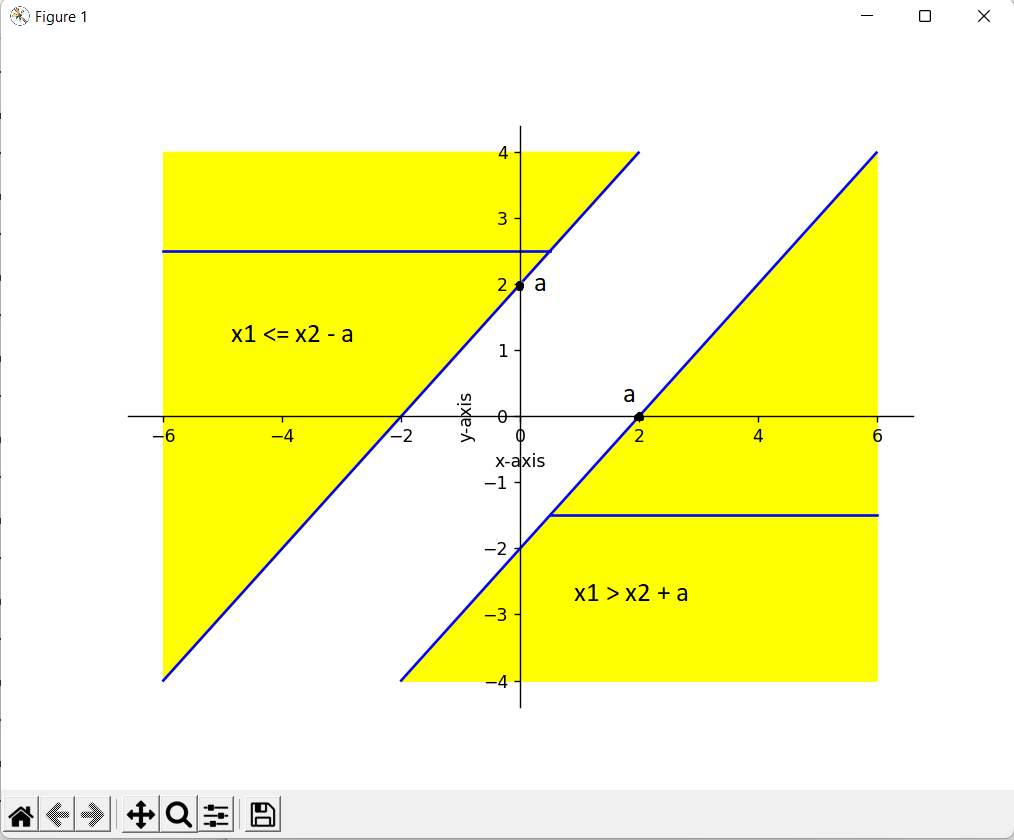
\includegraphics[width=\columnwidth]{fig.png}
            \caption{Required region}
            \label{fig.}
        \end{figure}
    \end{frame}
    \begin{frame}{Solution}
        In second order density of x(t)\\
        P\{$|x(t + \tau) - x(t)| \geq a $\} \\

        = $\int_{-\infty}^{\infty}\int_{-\infty}^{x_2 - a} f(x_1,x_2;\tau) \,dx_1\,dx_2 + \int_{-\infty}^{\infty}\int_{x_2 + a}^{\infty} f(x_1,x_2;\tau) \,dx_1\,dx_2$

         (This the region that we have plotted in previous slide)
    \end{frame}
\end{document}
